\chapter{Background}
\label{Chapt2}
\section{Introduction}

This chapter will explore the fundamental information relevant to this project, with an emphasis on the world of DNS abuse and transparency. It will include a thorough investigation of the domain name system (DNS), its crucial function in the online community, and the variety of abuses it faces. The history of the widely used policies and organisations aimed at stopping DNS abuse, including a thorough examination of the DNS Abuse Institute and its accomplishments, is essential to our investigation. A 'competition landscape' providing a critical examination of current market choices, from automated solutions to human tactics, will be provided as we navigate through the current methodology and technology deployed to detect and combat DNS abuse.  This analysis will also cover new developments that aim to improve DNS security and privacy, providing insight into the use and consequences of technologies like DNS over TLS (DoT) and DNS over HTTPS (DoH). The reader will obtain an in-depth understanding of the current situation of DNS abuse and the need for a more open, strong, and proactive strategy by analysing these various techniques and appreciating their strengths and weaknesses. This chapter emphasises the importance of the suggested solution in an era where digital authenticity is crucial, not only by providing information but also by laying the groundwork for its presentation as a better and essential progression in the battle against DNS abuse.

\section{Understanding DNS and Its Vulnerabilities}

The Domain Name System (DNS) is a crucial part of the infrastructure of the Internet, serving as the key that converts computer-understandable IP addresses into human-friendly domain names. Although the DNS plays a vital role in maintaining ongoing online activities, privacy and security problems still arise. The ScienceDirect paper "Domain Name System Security and Privacy: A Contemporary Survey" provides a thorough analysis of these concerns. This survey highlights the fundamental significance of the DNS while illuminating the weaknesses that malicious actors may take advantage of \cite*{sciencedirect2023dns}.

A variety of security threats exist, ranging from DNS infrastructure-targeting distributed denial of service (DDoS) assaults to cache poisoning and hijacking. Each of these attacks has the potential to do significant harm, including interruptions in service and the promotion of theft and spying. Due to the standard DNS design's lack of encryption, users' query data is vulnerable to misuse and eavesdropping, raising serious privacy problems. Still, weaknesses do not mark the end of the story. In the same survey, new approaches to improving DNS security and privacy are examined. The use of DNSSEC (DNS Security Extensions), which authenticates DNS data and guarantees its integrity while repelling some types of attack, is one example of these advances in cryptographic security measures. Moreover, privacy-enhancing technologies are being used to encrypt DNS queries, preventing eavesdropping and manipulation, such as DNS over HTTPS (DoH) and DNS over TLS (DoT).

The environment of DNS threats and defences is always changing in sync with the internet. For systems to be robust and resilient, it is essential to understand these weaknesses and the continuous efforts being made to mitigate them. An in-depth discussion of DNS vulnerability details, the effects of these safety concerns, and creative solutions that aim to bring in a new era of DNS security and privacy will be provided in this section \cite{sciencedirect2023dns}.

\section{Current efforts and organisations combatting DNS Abuse}

Addressing DNS abuse is a complex challenge that requires coordinated efforts across various sectors of the Internet ecosystem. Foremost among the entities dedicated to this cause is the DNS Abuse Institute. Established with a focused mission, the DNS Abuse Institute aims to combat DNS abuse and ensure the safety and security of the domain name system. Their goal is to assist the internet community in identifying, reporting, and mitigating instances of DNS abuse, thereby fostering a safer online environment \cite{dnsabuseinstitute2023}. The institute emphasizes the development and support of initiatives that enhance the understanding and mitigation of DNS abuse. They introduce innovative solutions like the "Compass Dashboards," which provide essential data and insights to registries and registrars, aiding them in making informed decisions to combat abuse. Furthermore, the DNS Abuse Institute is committed to transparency and education. They regularly publish reports and bulletins, such as the "DNSAI 2022 Annual Report" and the "DNSAI Bulletin 2023 04; Account Take Overs," offering a detailed view of the state of DNS abuse and the steps being taken to address it \cite{dnsabuseinstitute2023} . These publications serve as a valuable resource for stakeholders looking to understand the landscape of DNS abuse and the collective efforts to mitigate it  \cite{dnsai2022report}.

In addition to the DNS Abuse Institute, organizations like the Internet Corporation for Assigned Names and Numbers (ICANN) play a critical role in the global effort to monitor and reduce DNS abuse. ICANN's reports and initiatives provide insights and guidelines that shape policies and practices in the domain name industry. Their work involves collaboration with various stakeholders, including registries, registrars, and policy-making bodies, to develop and enforce standards that minimize DNS abuse while maintaining the openness and interoperability of the internet \cite{icann2022dnsabuse} . These organizations, along with numerous others involved in the fight against DNS abuse, contribute to a multi-faceted approach that includes policy development, technological innovation, and community engagement.\cite{dnsabuseinstitute2023} By highlighting the objectives, methods, and reports published by these entities  \cite{dnsai2022report}   , this section will provide a comprehensive view of the current efforts and organizations dedicated to combating DNS abuse, illustrating the collaborative nature of this ongoing battle \cite{icann2022dnsabuse} .

\section{DNS Privacy and Security Enhancements}

The digital world is changing, and so too is the need for enhanced privacy and security measures within the Domain Name System (DNS). Significant advancements have been made to protect users and their data, particularly through the implementation of DNS over TLS (DoT) and DNS over HTTPS (DoH). These technologies represent a paradigm shift in DNS query encryption, aiming to address privacy concerns and secure communication between clients and servers. DNS over TLS (DoT) offers a way to encrypt DNS requests and answers, making it harder for bad actors to simply intercept or change the data. This technology is essential for protecting user privacy and stopping man-in-the-middle and eavesdropping attacks. In the same way, DNS over HTTPS (DoH) leverages the security features and broad acceptance of HTTPS to protect DNS requests within the HTTPS protocol, adding an extra degree of protection.

The paper "DNS Privacy in Practice and Preparation," focusing on how these technologies are being accepted and put into effect, provides an in-depth review of these developments. It emphasises how important DoT and DoH are to protecting DNS privacy and how key public DNS service providers are supporting these more and more. The implementation of DoT and DoH is not without difficulties, regardless of their advantages. Their effectiveness depends on factors like performance concerns and the requirement for extensive implementation across multiple platforms. The study also highlights how critical TCP Fast Open (TFO) is to lowering TCP-based DNS query latency, which is essential for balancing privacy and speed  \cite{acm2023dnsprivacy}  .


\section{Different Forms of DNS Abuse}

DNS abuse takes many forms, each with its procedures and effects on users and the internet as a whole. It is essential to understand these various pieces of evidence to create responses and regulations that work. This section will examine the comprehensive analysis of DNS abuse as presented, going into the description, mechanism, and impact of each kind.

\subsection{Phishing}
\begin{itemize}
    \item \textbf{Description:} Phishing is a technique aimed at deceiving individuals by creating website addresses that mimic those of companies, to trick users into revealing sensitive information such as login credentials, credit card numbers, or personal identification information.\cite{webinarcare2023dnsstats}
    \item \textbf{Mechanism:} This deception often occurs through emails or messaging services that direct users to websites resembling authentic ones.\cite{jakobsson2006phishing}
    \item \textbf{Impact:} Victims may suffer identity theft, financial fraud, and security compromise.
\end{itemize}

\subsection{Confusable Domains (Typosquatting)}
\begin{itemize}
    \item \textbf{Description:} Registering domain names that look visually similar to popular websites, taking advantage of typing errors or character similarities.\cite{inta2023dnstypo}
    \item \textbf{Mechanism:} Users may accidentally visit these websites when making a typo in a URL, potentially exposing them to malware or phishing attempts.
    \item \textbf{Impact:} Deception of users and potential harm to brand reputation.\cite{edelman2008typosquatting}
\end{itemize}

\subsection{Domain Hijacking}
\begin{itemize}
    \item \textbf{Description:} Unauthorized acquisition of domain names by exploiting security vulnerabilities in the domain registration system.\cite{inta2023dnstypo}
    \item \textbf{Mechanism:} Attackers may use tactics like social engineering, phishing, or exploiting security loopholes to gain control over a domain.
    \item \textbf{Impact:} Loss of website control, redirection to malicious sites, and potential data breaches.
\end{itemize}

\subsection{Botnets}
\begin{itemize}
    \item \textbf{Description:} Botnets involve controlling a group of computers infected with malware, used to carry out attacks or spread spam and malware.\cite{citpyour}
    \item \textbf{Mechanism:} Malware infects unsuspecting users’ computers, incorporating them into a network under the attacker's control.
    \item \textbf{Impact:} Can result in large-scale DDoS attacks, mass spam campaigns, and widespread malware dissemination.
\end{itemize}

\subsection{Fast Flux Hosting}
\begin{itemize}
    \item \textbf{Description:} A technique used to conceal the location of websites associated with phishing and malware distribution.\cite{lin2013genetic}
    \item \textbf{Mechanism:} Involves a network of compromised hosts that regularly modify DNS records to evade detection.
    \item \textbf{Impact:} Makes tracking and shutting down malicious sites difficult.
\end{itemize}

\subsection{Domain Generation Algorithms (DGA)}
\begin{itemize}
    \item \textbf{Description:} DGAs generate domain names that act as meeting points for botnets.\cite{antonakakis2012throw}
    \item \textbf{Mechanism:} Malicious software uses algorithms to generate a sequence of domain names for command-and-control servers.
    \item \textbf{Impact:} Adds complexity to efforts aimed at disrupting botnet command and control channels.
\end{itemize}

\section{How DNS Abuse Harms Users}

DNS abuse has serious and detrimental effects for both users and organisations, going beyond basic technological disruptions. Identity theft is among the most direct and direct effects. Phishing attacks, a frequent type of DNS abuse, use realistic-looking websites to trick visitors into revealing sensitive data. Such attacks can yield information that results in financial theft, unauthorised access to accounts, and long-term harm to a person's reputation and credit

\subsection{Identity Theft}
\begin{itemize}
    \item \textbf{Phishing:} Phishing attacks often use domain names that imitate legitimate websites, fooling users into providing sensitive information such as usernames, passwords, or financial details, leading to potential identity theft.\cite{godaddy2023dnsabuse, jakobsson2006phishing}
\end{itemize}

\subsection{Financial Loss}
\begin{itemize}
    \item \textbf{Deceptive Transactions:} Users may be tricked into making payments to deceptive websites or unknowingly disclose their credit card information, resulting in financial losses.\cite{godaddy2023dnsabuse, bohme2013economics}
\end{itemize}

\subsection{Data Breach}
\begin{itemize}
    \item \textbf{Malware:} Malicious software spread through compromised DNS systems can allow unauthorized access to corporate data, leading to data breaches.\cite{icann2022dnsabusetrends, fowler2016data}
\end{itemize}

\subsection{System Compromise}
\begin{itemize}
    \item \textbf{Malware Infection:} Systems infected with malware due to DNS abuse can be exploited for further attacks, including the creation of botnets or the distribution of ransomware, resulting in system compromise.\cite{dotmagazine2022dnsabuse, saxe2018malware}
\end{itemize}

\section{Future Dangers of DNS Abuse}

As technology develops, so do cyber attackers' strategies and tools, creating a dynamic environment for DNS abuse that could present new risks in the future. The sophistication of attacks has increased, which is a major issue. Cybercriminals are always creating increasingly sophisticated methods to take advantage of DNS, like creating phishing schemes that are more convincing and utilising complex virus distribution networks

\subsection{Increased Sophistication}
\begin{itemize}
    \item \textbf{Evolving Techniques:} Cyber attackers are constantly developing more sophisticated techniques to exploit DNS, such as advanced phishing schemes and malware distribution.\cite{icann2022dnsabusetrends, wrightson2014advanced}
\end{itemize}

\subsection{IoT Vulnerabilities}
\begin{itemize}
    \item \textbf{Expanding Vulnerabilities:} The widespread adoption of Internet of Things (IoT) devices, which often lack robust security measures, presents a growing target for DNS-based attacks.\cite{circleid2020dnstrends, mahmoud2015internet}
\end{itemize}

\subsection{Infrastructure Attacks}
\begin{itemize}
    \item \textbf{DNS as a Prime Target:} Attacks on DNS infrastructure can disrupt internet services on a large scale, including DDoS attacks targeting DNS providers or exploiting weaknesses in DNS protocols.\cite{dotmagazine2022dnsabuse, dooley2017dns}
\end{itemize}

\subsection{Deepfakes and AI}
\begin{itemize}
    \item \textbf{AI-Enhanced Phishing:} The use of AI technologies, such as deepfakes, has made phishing attacks more convincing and deceptive, manipulating audio and video content to impersonate trusted entities.\cite{icann2022dnsabusetrends, schick2020deep}
\end{itemize}

\subsection{Cloud Computing Vulnerabilities}
\begin{itemize}
    \item \textbf{Targeting Cloud Services:} As organizations increasingly rely on cloud-based services, cybercriminals are exploiting DNS vulnerabilities to attack these platforms, potentially leading to data breaches and service disruptions.\cite{mather2009cloud}
\end{itemize}

\subsection{Mobile Device Exploitation}
\begin{itemize}
    \item \textbf{Mobile DNS Attacks:} The rising usage of mobile devices has led cybercriminals to target smartphones and tablets through DNS-based attacks, which can lead to data theft and the spread of malware.\cite{au2016mobile}
\end{itemize}

\subsection{Cryptocurrency and Blockchain Exploitation}
\begin{itemize}
    \item \textbf{Crypto-Related DNS Attacks:} Attackers could exploit DNS vulnerabilities to redirect users to fake cryptocurrency exchanges or blockchain platforms, leading to financial fraud and theft of digital assets.\cite{bashir2019advanced}
\end{itemize}

\subsection{Political and Information Warfare}
\begin{itemize}
    \item \textbf{DNS in Cyber Warfare:} The manipulation of domain name systems can be used to spread misinformation or disrupt services during significant political events, serving as a tool for political and information warfare.\cite{chapple2021cyberwarfare}
\end{itemize}

\subsection{Exploiting Emerging Technologies}
\begin{itemize}
    \item \textbf{Abuse in New Tech Domains:} As new technologies such as 5G, AI, and quantum computing advance, tactics involving DNS abuse are likely to evolve, potentially leading to more sophisticated attacks.\cite{brunner2021cybersecurity}
\end{itemize}

\subsection{Supply Chain Attacks}
\begin{itemize}
    \item \textbf{DNS in Supply Chain Compromise:} DNS manipulation can also be employed as part of supply chain attacks, targeting software updates or cloud-based services to compromise organizations.\cite{boyson2014cyber}
\end{itemize}

By understanding these future dangers and emerging trends, stakeholders can better prepare and adapt their strategies to anticipate and counteract the evolving nature of DNS abuse.


\section{Mitigation Strategies and Best Practices }

To address the broad nature of the threats, combating DNS abuse requires an integrated strategy that integrates multiple strategies and best practices. Setting up procedures for reporting and monitoring is one fundamental tactic. Automated systems have the capability to track domain name registration patterns that may indicate DNS abuse, and protocols for reporting questionable actions can help ensure prompt intervention \cite{icannndnssec} . In order to confirm security and make sure systems have not been compromised, regular audits of DNS setups and domain registrations are also necessary \cite{lucas2021tls} .

\begin{enumerate}
    \item \textbf{Monitoring and Reporting}
    \begin{itemize}
        \item Implementation: Use automated systems to monitor the registration of domain names for patterns that may indicate DNS abuse \cite{icannndnssec}. Establish procedures for reporting activities to authorities or cybersecurity organizations \cite{lucas2021tls}.
    \end{itemize}
    \item \textbf{Security Awareness Training}
    \begin{itemize}
        \item Implementation: Develop training programs for users and IT staff with a focus on recognizing phishing attempts, practicing browsing habits, and understanding DNS security.
    \end{itemize}
    \item \textbf{DNS Security Extensions (DNSSEC)}
    \begin{itemize}
        \item Implementation: Deploy DNSSEC to ensure the integrity of DNS data. This involves signing DNS records to protect against modifications and DNS spoofing.
    \end{itemize}
    \item \textbf{Multi-Factor Authentication (MFA)}
    \begin{itemize}
        \item Implementation: Enforce Multi-Factor Authentication (MFA) for domain registrars and interfaces used for managing DNS \cite{icannndnssec}. This adds a layer of security beyond passwords, helping prevent unauthorized domain transfers or alterations \cite{moghaddam2014ecco}.
    \end{itemize}
    \item \textbf{Blacklisting and Takedown Services}
    \begin{itemize}
        \item Implementation: Collaborate with cybersecurity firms to identify and blacklist domains engaged in malicious activities. Establish response teams dedicated to taking down domains involved in DNS abuse.
    \end{itemize}
    \item \textbf{Collaboration}
    \begin{itemize}
        \item Implementation: Foster collaboration among internet service providers (ISPs), domain registrars, governments, and cybersecurity organizations. Share intelligence and best practices to collectively enhance defense against DNS abuse \cite{skopik2017collaborative}.
    \end{itemize}
    \item \textbf{Regular Audits}
    \begin{itemize}
        \item Implementation: Conduct security audits of domain registrations and DNS configurations to verify their security and ensure they have not been compromised \cite{coronado2014auditing}.
    \end{itemize}
    \item \textbf{Machine Learning}
    \begin{itemize}
        \item Implementation: Utilize AI and machine learning algorithms to analyze patterns in DNS traffic and proactively predict instances of DNS abuse \cite{icannndnssec}. This proactive approach enables the identification of threats before they materialize \cite{tsukerman2019machine}.
    \end{itemize}
    \item \textbf{Geo-Blocking and IP Filtering}
    \begin{itemize}
        \item Implementation: Deploy geo-blocking and IP filtering techniques to limit access to DNS services from regions that have a history of DNS abuse. This can reduce the risk of attackers utilizing these services to carry out malicious activities or distribute malware \cite{meeseedited}.
    \end{itemize}
    \item \textbf{Enhanced Domain Validation Procedures}
    \begin{itemize}
        \item Implementation: Enhance the domain registration process by implementing validation procedures. This may involve verifying the identity of individuals or organizations registering domains, especially for domains that resemble brands or fall into sensitive categories. By taking these measures, we can strengthen security and mitigate risks associated with fraudulent domain registrations.
    \end{itemize}
\end{enumerate}

Each of these strategies plays a crucial role in creating a comprehensive defense against DNS abuse. By integrating these tactics, organizations can establish robust, proactive measures to detect, prevent, and mitigate the ever-evolving threats posed by DNS abuse.

\section{Summary and Synthesis}

This chapter has examined all aspects of DNS abuse,  the various forms, the serious harm it does, as well as potential future threats and new trends. To create efficient regulations and countermeasures, it is essential to comprehend the extent and consequences of DNS abuse. The conversation emphasised DNS's vital function in the digital ecosystem as well as its susceptibility to misuse.Significant progress towards resolving these issues has been made by organisations like the DNS Abuse Institute and ICANN, as well as developments in DNS privacy and security technologies like DoT and DoH. Yet as new technologies are incorporated into the equation and the threat environment changes in sophistication, it becomes more and more important to adopt alert, flexible, and cooperative strategies.  

A road map for preventing DNS abuse is provided by the mitigation techniques and best practices discussed in this chapter. Every tactic contributes to a defence mechanism, from advanced technology solutions and improved methods for validation to monitoring and reporting. It is impossible to overestimate the value of cooperation, regular checks, and the application of cutting-edge technologies in anticipating and stopping DNS abuse. After analysing the data, it is evident that a team effort is needed to comprehend, track, and mitigate DNS abuse. A complex strategy that integrates multiple techniques and encourages collaboration across industries is required instead of a single, insufficient strategy. Our approaches to preserving the integrity and security of the DNS and, consequently, the larger internet infrastructure, must adapt as the digital environment does.

By understanding the connections between different aspects of DNS abuse and reinforcing the collective effort required for effective mitigation, stakeholders can be better prepared to face the challenges ahead. This chapter sets the stage for further research and action, aiming to contribute to a safer, more secure digital world.

\section{Future Research and Development}

It is more important than ever to conduct ongoing study and development as we navigate the ever-changing arena of DNS abuse. Future work must concentrate on comprehending new threats and creating creative countermeasures. The following are some recommended areas for additional study and possible advancements in the fight against DNS abuse:

I will come back to this chapter after I am done with my thesis 

\chapter{State of the Art}

This Chapter explores the strategies being employed to prevent DNS abuse as well as new developments in this field. It explores and evaluates the effectiveness and transparency of multiple mitigation techniques, including DNS filtering and threat intelligence. Additionally, the use of domain generating techniques and DNS tunnelling are two novel forms of DNS abuse that are highlighted in this section. Along with the difficulties in guaranteeing openness in these methods, the role of AI and machine learning in identifying and stopping DNS abuse is covered. The final half of the section includes a discussion on potential future research areas and technologies to improve DNS security. Case studies offer practical insights into DNS abuse occurrences. This in-depth analysis is an invaluable tool for comprehending how DNS abuse is changing and the continuous efforts to combat it.


\section{Current Strategies and Their Effectiveness in Relation to DNS Abuse}

Currently, ways to stop DNS misuse are very important in keeping the internet's system for domain names safe. These plans are about stopping bad websites, learning about threats, discovering strange behaviors, and attempting to find and stop wrong actions. DNS filtering is a way to stop or allow access to certain websites. Threat intelligence uses data analysis to find out possible risks \cite{schmid2021thirty}. Finding unusual DNS activities that suggest bad intentions is what anomaly detection does. But, sometimes, these methods don't work right. They face issues like errors and require quick access to vital data about dangers. It is very important to see how well or poorly DNS abuse prevention methods work. This helps make them better.

\subsection{Mitigation Strategies}

The best ways to stop the wrong use of DNS are by using a tool to block, knowing about dangers, and finding strange stuff. DNS filtering is like stopping or allowing someone to visit certain websites based on rules first. The main job of threat intelligence is to find possible dangers and spot strange activities in the DNS \cite{rizvi2022application} You need to carefully look at every plan to understand what it is good or bad and how well works in real life. For example, using DNS filtering can sometimes let bad things get through. This might end good websites and make the user feel bad. How well threat intelligence works depends on how fast and accurate the data it uses is. It's hard to find strange acts because sometimes it can't tell the difference between bad actions and usual things done in a new way.

\subsection{Evaluation of Transparency}

It's super important to demonstrate how individuals can stop misuse of DNS. This helps create trust with important people, such as internet users, businesses, and those who lead. Easy ways to do things show responsibility and make people work together to stop wrong use. The test for openness should consider things like ways we clearly talk about stopping bad actions, sharing wrong results, and making information easily available about how choices were made \cite{chaganti2023survey} Groups that share their goals frequently share updates and talk with the public to help make a clear DNS system.

\section{Emerging Trends in DNS Abuse}

New methods of using DNS wrongly are changing how secure we are online. They create new issues and weaknesses. These patterns include complicated methods of causing harm, such as DNS tunneling. This is when bad people hide normal internet traffic in DNS packets to dodge getting caught. Also, the increase in domain creation methods (DGAs) is a big risk \cite{kapoor2021ransomware}. These systems make a lot of domains that look random, making it difficult to guess which ones could be dangerous. As the DNS system changes, those in computer security need to know these new trends. Good plans and future actions must always be made better to fight these changing ways of misusing DNS. They need to defend the trust in internet systems well.

\subsection{New Forms of DNS Abuse}

In the changing world of computer protection, new ways to use DNS wrongly keep testing old ways of stopping undesirable acts. A new danger is DNS tunneling. This is when bad people use the DNS system to hide traffic that is not part of the DNS. This allows them to speak quietly and stay hidden. One more problem is the use of domain generation algorithms (DGAs). These help bad internet people make lots of random-looking domains \cite{kaur2023artificial}. This makes it tough to guess and stop bad websites properly. Also, incorrectly using subdomains is a lasting problem. Bad guys hide their actions on good websites with smaller parts, making it hard to find them. It's very important for people who work in cybersecurity to get used to these changing ways of wrong use.

\subsection{Predictive Measures and Their Transparency}

Preventing DNS abuse measures are designed to stop it right away. Complex systems and smart machine learning figure out bad behavior patterns. Staying calm and sharing these decisions about the future is very important. This lets us understand how decisions are made and makes sure that good folks are kept responsible \cite{hussain2022software}. It's important to explain why predictions are made, as it shows the reason for them, tells what data was used to learn, and gives suggestions about how decisions are made. It's tough to find the perfect balance between how complicated foreseeing models are and how easy they are to grasp.

\section{Technological Advancements}

Improvements in technology, especially using AI and machine learning to fight DNS abuse, are changing how things are done. AI and machine learning are very important in finding and stopping DNS misuse. These tools use automatic systems and good pattern understanding to quickly check large amounts of data \cite{goethals2021enabling}. This helps us spot even little bad habits, too. But, when AI and machine learning work together, it can be difficult to see how things work. Some complicated computer programs are like a mystery box, making people scared about how to understand them. People have to find a good balance between difficulty in identifying danger and clarity in being responsible.

\subsection{Role of AI and Machine Learning}

Fighting DNS abuse with AI and machine learning is important. It's a new way to find and stop dangers before they become a problem. These tools assist groups to examine large amounts of data quickly, discovering hidden patterns in the internet's domain name system that reveal bad behavior. AI's ability to learn from past data lets it see changing attack methods. This helps to find threats easier \cite{tariq2023critical}. Machine learning models, which can change, help us find issues early and respond fast. This makes the whole DNS system stronger. Even though they give hope, there are still obstacles that make things hard to understand clearly. This needs a careful balance between how hard things are and who can be held accountable.

\subsection{DNS Abuse Transparency Challenges with AI and Machine Learning}

AI and machine learning can help make DNS abuse prevention better, but experts need to fix issues by being clear. People are worried about understanding why complex systems make choices because of the "black box" part. It is important to understand how AI models make certain decisions. This helps build trust and makes sure people are responsible for them. There are difficulties in making things clear, such as needing to write down what data was used for training, telling others about the things that affect choices, and explaining how models change to face new risks. It's still hard to find the right balance between the complexity needed for good threat detection and the openness needed for blame.

\section{Case Studies and Real-World Applications}

In the past few years, technology has become so widespread that we have witnessed an unmatched number and complexity of cyber threats. A significant vulnerability that can be exploited is the Domain Name System DNS, a critical part of internet infrastructure that translates human-readable names into IP addresses \cite{kumari2021sac115}. In this case, the study completely analyze one specific company, XYZ Corporation, as an example of DNS abuse in the real-world environment and analyze all details through figures, graphs, and charts. This abuse of DNS took place as a prolonged campaign against XYZ Corporation, a multinational technology conglomerate \cite{mohammed2021network}. Attackers used weaknesses in the company's DNS infrastructure to perform various malicious activities, including domain hijacking, DNS tunneling, and DDoS attacks. A timeline graph was also prepared to see the scale of abuse and how the attacks progressed with each event that occurred in the organization as shown in Figure \ref{fig:figureOne}.

\begin{figure}[ht]
\centering
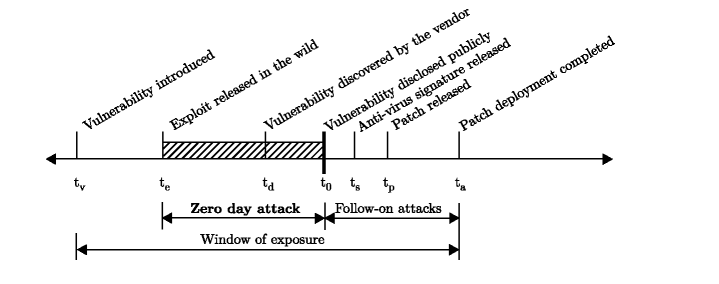
\includegraphics{background/XYZ1.png}
\caption{Timeline of DNS Abuse Attacks on XYZ Corporation}
\label{fig:figureOne}
\end{figure}

The relationship between this correlation raises questions about the attackers' understanding of the inner workings of the firm, as well as insider threats. A closer analysis of the DNS abuse types employed by such offenders revealed that domain hijacking was common \cite{bayer2022study}. Figure \ref{fig:figureTwo} shows how diverse DNS abuse techniques were used in the XYZ Corporation case, and domain hijacking was significantly higher than all other methods combined.

\begin{figure}[ht]
\centering
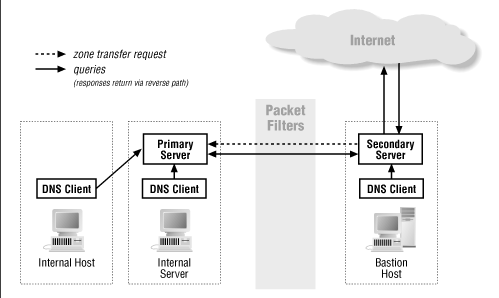
\includegraphics{background/XYZ2.png}
\caption{Distribution of DNS Abuse Techniques Against XYZ Corporation}
\label{fig:figureTwo}
\end{figure}

There is a domain hijacking technique where the attackers may effectively take control over a company without authorization; domain hijacking is one of the major threats to the organizations that are affected. The figure shows that strong Security is key to preventing unauthorized access to domain registration accounts; favoring multi-factor authentication is the way of keeping these attacks away \cite{paz2020cyber}. This case study sheds light on the subtleties of DNS abuse as it targeted XYZ Corporation, showing the importance of understanding and dealing with an unpredictable cyber threat environment. The figures, graphs, and charts serve to illustrate the attack procedures for safeguards and give credence to the notion that an all-encompassing cybersecurity strategy is integral to preventing DNS abuse in the networked digital environment of our day.

\section{Challenges and Future Directions}

When dealing with issues about DNS misuse, big issues are quick changes in new threats, the need for global teamwork right away, and the constant use of technology. Fixing the balance between lies and truth, getting better at recognizing threats, and overcoming old tech limits remain very hard tasks. In the future, scientists should try to make technology better \cite{pour2023comprehensive}. This means making AI models better at understanding what's happening in DNS traffic. This also means finding ways to use blockchains for better protection when registering domains. Concentrating on using local tools could offer new methods to safeguard the DNS system. Key persons, quick shifts to new threats, and discovering new answers will be very important in deciding how to manage DNS abuse in the future.


\subsection{Identification of Current Challenges}

It's really important to find ways to stop misuse of DNS. This will aid in crafting clever responses and improve things continually. A big problem is handling threats that change and adapt over time. As naughty people on the internet change how they fool others, we need to change how people stop the wrong use of DNS \cite{bhattacharya2023dns}. This will require constant effort to make new plans and update old ones. One big issue in working together globally is making contact with people from all over the world. The internet works everywhere, and misusing DNS is a problem everywhere in the world. Experts have to join forces to fix this issue \cite{altulaihan2022cybersecurity}. Putting together many rules and laws and ways to follow them is a tough task. It needs careful thinking and teamwork. A big issue is an ongoing struggle to find a balance between reducing wrong positive and negative outcomes. People need easy methods to stop bad things on the internet while also not interrupting good internetwork. Fixing this careful balance is still a major issue. Big plans can spoil user experiences \cite{lyu2022survey}. But, if something is too simple, bad behavior might not be seen. As DNS misuse changes, we have to solve these issues. This will improve and make our methods against it better and stronger.

\subsection{Discussion on Future Research Directions and Technologies}

When planning to stop the misuse of DNS in the future, discussing new research ideas and upcoming technology is crucial. The always-changing state of internet threats needs us to continually create new things. This is so people can stay one step ahead of the bad people. Future work on DNS abuse needs to start by building better tools. These can help tackle how bad guys on the internet keep changing their tricks \cite{bovenzi2023blockchain}. This means we need to look at more complex AI and machine learning tools that can understand the details of web traffic. This will make the results more accurate and stop wrong signals from being sent. Moreover, there is a rising need to use blockchain tech to make domain registration safer and stop any bad or harmful changes. People should have easy methods to report bad use of DNS. This will make sure everyone knows about dangers and how to fix them easily \cite{gu2021iot}. Working together in the world is very important because computer dangers go beyond borders. So, everyone around the world needs to work together. The discussion about where research needs to go in the future highlights the importance of working together. The DNS system should have better technology, work as a team, and have agreed-upon methods to make it strong against smart ways of misuse.


\section{Conclusion}

The wrong use of DNS keeps being a big issue. Present plans, while sometimes useful, require constant adjustment and getting better. It's key to have solutions for fixing issues available. This helps build trust and work well with those involved. Abusing DNS in new ways brings fresh issues that require clever solutions. AI and machine learning can help find things, but we need to show how they work better so people can keep bad people in check. Learning from real-life situations teaches us a lot about good and bad ways of being open. This helps us create the best methods for our business. There are still issues with showing and stopping the wrong use of DNS. People need to keep learning and working as a team. People should focus on making better technology, joining forces with other nations, and using common methods of sharing information in the future. As the internet changes, we must stay active and work together to stay ahead of bad people who want to hurt us. This will make sure that the DNS is secure.

\section{Summary of Findings}

The study about the bad use of DNS looked at current ways, checked new trends, talked about tech advancements, and explored real examples in life. Checking for secret ways in plans to stop DNS abuse showed the value of clear communication and honesty in building trust with the community. People are finding new ways to misuse the DNS system and guess it. People have to keep making new things, so they don't get caught by changing dangers. Improvements in technology, especially with AI and learning machines, showed how automation can make it easier to spot dangers. But it also made things harder to understand, and this needs careful looking at. Examples from real life showed what did and did not work in making DNS abuse clearer. These provided essential advice for the business. Issues with making things clear and stopping wrong actions were found. This shows how much it matters to keep learning and working with others. In the future, discussing issues and future plans will show the need for creative studies, help from other nations, and common ways to share information. The approach in this paper that stresses action and working together is really important to handle the changing pattern of DNS abuse. It's also important to keep the DNS system safe and secure.



























\section{Figures}
Graphs, pictures and other images should be included in your report as a numbered, captioned figure. An example is given in Figure \ref{veldis}.

%%%%%%%%%%%%%%%%%%%%%%%%%%%%%%%%%%%%%%%%
\begin{figure}[h]
      \centering
      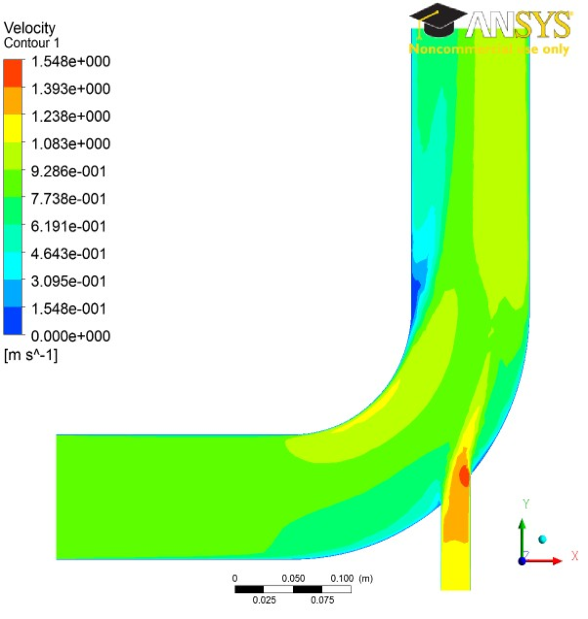
\includegraphics{background/5e1-1.pdf}
      \caption{Velocity distribution on the mid-plane for an inlet velocity for case 1.}
      \label{veldis}
\end{figure}
%%%%%%%%%%%%%%%%%%%%%%%%%%%%%%%%%%%%%%%%

The figure and caption should be centred. The figure numbering starts at 1 at the beginning of each chapter. The caption should provide a brief description of what is being shown. The figure should appear in the document after it is referred to in the text. No figure should be included which is not referred to in the text. Ensure that the size and resolution of images imported from software are sufficient to read any text.

\section{Tables}
Tables are an important way of displaying your results. Table \ref{tab:treatments} is a sample table, adapted from the Master/Doctoral Thesis template at \url{http://www.latextemplates.com/cat/theses}, which was generated with this code:

{\footnotesize
\begin{verbatim}
\begin{table}[b]
\caption{The effects of treatments X and Y on the four groups studied.}
\label{tab:treatments}
\centering
\begin{tabular}{l l l}
\toprule
\textbf{Groups} & \textbf{Treatment X} & \textbf{Treatment Y} \\\midrule
1 & 0.2 & 0.8\\
2 & 0.17 & 0.7\\
3 & 0.24 & 0.75\\
4 & 0.68 & 0.3\\
\bottomrule\\
\end{tabular}
\end{table}
\end{verbatim}
}

\begin{table}[b]
\caption{The effects of treatments X and Y on the four groups studied.}
\label{tab:treatments}
\centering
\begin{tabular}{l l l}
\toprule
\textbf{Groups} & \textbf{Treatment X} & \textbf{Treatment Y} \\
\midrule
1 & 0.2 & 0.8\\
2 & 0.17 & 0.7\\
3 & 0.24 & 0.75\\
4 & 0.68 & 0.3\\
\bottomrule\\
\end{tabular}
\end{table}

Tables are numbered in the same way as figures. Typically tables also have a short caption, but this is not universally true. The number and caption appear above the table, not below as with figures. Again, no table should appear in the report which has not been referred to in the text. Tables should come after they are discussed in the text. The exact formatting of the table depends somewhat on the content of the table, but in general, the text in the table should be the same font and size as the main text. 

\section{Equations}
All equations should be numbered sequentially. The numbering restarts automatically at the beginning of each chapter, and contains the number of the chapter alongside the equation number. Unlike figures and tables, you may not need to refer to every equation in the text. You should take care to format equations properly. Do no simply try to use plain text. Use the equation layout facilities. An example of how equations should appear is shown in \eqref{sampleequation}. Here is the code for it:

{\footnotesize
\begin{verbatim}
\begin{equation}
\textrm{div}(\underline{u}) = \frac{\delta u}{\delta x} + \frac{\delta v}{\delta y} +
        \frac{\delta w}{\delta z} = 0
\label{sampleequation}
\end{equation} 
\end{verbatim}
}

\begin{equation}
\textrm{div}(\underline{u}) = \frac{\delta u}{\delta x} + \frac{\delta v}{\delta y} + \frac{\delta w}{\delta z} = 0
\label{sampleequation}
\end{equation} 

\section{Referencing published work}
It is important to give appropriate credit to other people for the work that they have shared through publications. In fact, you must sign a declaration in your report stating that you understand the nature of plagiarism. As well as avoiding plagiarism, citing results or data from the literature can strengthen your argument, provide a favourable comparison for your results, or even demonstrate how superior your work is.

There are many styles to reference published work. For example, the parenthetical style (which is also called the \emph{Harvard style}) uses the author and date of publication (e.g. ``Smith and Jones, 2001''). There is also the Vancouver style (or the \emph{citation sequence style}). In the IEEE style, which is used in this document in the default setup, the publications are cited using bracketed numbers which refer to the list in the References section at the end of the report. The references are listed in the order that they are cited in the report. A variant is \emph{name sequence style}, in which the publications are referenced by number, but the list is arranged alphabetically. The following paragraph shows the use of the IEEE style: 

\begin{quote}
Several studies have examined the sound field around tandem cylinders generated by flow\cite{fitzpatrick2003flow,finnegan2010experimental}, while other investigations have focused on the effect of an applied sound field on the flow\cite{hall2003vortex}. Papers from conference proceedings\cite{jordan2001array}, books\cite{paidoussis2010fluid} and technical reports\cite{reyes2007power} can be dealt with in the same style.
\end{quote}

The IEEE style has the advantage that it is a little more compact in the text and does not distract from the flow of the sentence if there are a lot of citations. However, it has the disadvantage that it is not immediately clear to the reader what particular work has been referenced. You can use author names directly and discuss the work of Finnegan et al. \cite{finnegan2010experimental} similar to this sentence to make it more readable. 

It actually does not matter which particular referencing style is used as long as three important considerations are observed:
\begin{itemize}
\item the referencing style used throughout the document is consistent;
\item all material used or discussed in the text is properly cited;
\item nothing is included in the reference list that has not been cited.
\end{itemize}

Check with your supervisor as they may have a strong opinion on what you should use

This template has a suitable referencing style already set up -- you should use it and use the built-in BibTeX system to manage your references. See above for examples of how to cite a reference and look in the \texttt{sample.bib} file to see BibTeX references. It is strongly recommended that you use a bibliographic tool, such as EndNote (check out https://www.tcd.ie/library/support/endnote/), as this will facilitate compliance with these three requirements. Endnote can help you build you .bib file. Remember \href{http://scholar.google.com}{Google Scholar} and other search engines will give you BibTeX references for lots of academic publications. Be aware that Web of Science is more reliable for giving the full record for the BibTeX entry. Otherwise, you can easily make up your own based on the examples in that file.